\chapter[Working with Limits]{Working with Limits: Slutsky, the Continuous Mapping Theorem and the Delta Method}
\label{ch:limit-tools}

\begin{chaptergoals}
\begin{itemize}[nosep]
\item Which arithmetic survives a limit: sums, products and quotients for convergence in probability, and the one case (Slutsky's theorem) where it works for convergence in distribution.
\item The continuous mapping theorem: a continuous function of a convergent sequence converges.
\item The delta method: the Central Limit Theorem for a function of an average, with the derivative as the scale factor.
\item A map from every asymptotic result in the rest of the book back to these tools.
\end{itemize}
You now have two limits in hand: $\bar{X}_n \convp \mu$ from \cref{ch:lln} and $\sqrt{n}(\bar{X}_n - \mu) \convd \Gauss(0, \sigma^2)$ from \cref{ch:clt}. Almost nothing in statistics is literally an average, so the question is what you may do to these limits and still know where you end up.
\end{chaptergoals}

\section{Arithmetic and convergence}
\label{sec:conv-operations}

For convergence in probability and convergence almost surely, the arithmetic properties of limits of real-valued sequences have analogous arithmetic properties.
(Almost sure convergence is defined in \cref{app:modes}; on the minimal path, read the rules below for convergence in probability, the only one of the two the rest of the book uses.)

Let $(X_n)_{n \geq 1}$ and $(Y_n)_{n \geq 1}$ be sequences of r.v.s and suppose that:
\[
X_n \convasp X \text{ and } Y_n \convasp Y.
\]

Then:
\begin{enumerate}
\item \textbf{Additive property:} $X_n + Y_n \convasp X + Y$.

\item \textbf{Multiplicative property:} $X_n Y_n \convasp XY$.

\item \textbf{Division property:} If $Y \neq 0$ almost surely, then:
\[
\frac{X_n}{Y_n} \convasp \frac{X}{Y}.
\]
\end{enumerate}

For almost sure convergence these are just the calculus rules applied outcome by outcome: on the probability-one set where both sequences of numbers converge, their sums, products and quotients converge to the sums, products and quotients of the limits.
For convergence in probability the rules hold too, though the proof is a little longer.

\textbf{NB:} These rules \textbf{don't} apply to convergence in distribution.
The pitfall box in \cref{sec:conv-dist} gave the counterexample: $X_n = -Z$ and $Y_n = Z$ both converge in distribution to $\Gauss(0,1)$, but $X_n + Y_n = 0$, while two independent sequences with the same marginal limits would have sum converging to $\Gauss(0,2)$.
The marginal limits don't determine the limit of the sum because they say nothing about how $X_n$ and $Y_n$ are related.
This is where Slutsky's theorem comes in: it's the special case where one of the two limits is a constant, so there's no relationship to worry about.

\begin{bridge}[variances add, standard deviations do not]
An introductory course combines independent random variables with the rule `variances add': $\var(X \pm Y) = \var(X) + \var(Y)$, for a difference as well as a sum.
Without independence there is a third term, $\var(X \pm Y) = \var(X) + \var(Y) \pm 2\cov(X, Y)$, and the covariance is one part of the relation between $X_n$ and $Y_n$ that the marginal limits leave out.
In the counterexample above both variables have variance $1$: $X_n = -Y_n$ gives $\var(X_n + Y_n) = 0$, independence gives $2$, and $X_n = Y_n$ gives $4$, the case in which the standard deviations add, $1 + 1 = 2$.
Independence is the hypothesis behind the two-sample standard error $\sqrt{s_1^2/n_1 + s_2^2/n_2}$: two independent kiss studies of $124$ couples give two sample proportions with standard error $0.043$ each, and their difference has standard error $\sqrt{0.043^2 + 0.043^2} = 0.061$, not $0.086$.
Before-and-after measurements on the same subjects are usually positively correlated, so the two-sample formula overstates the variance of their difference, and the paired analysis of an introductory course works with the differences instead.
\end{bridge}

\section{Slutsky's theorem}
\label{sec:slutsky}

For convergence in distribution, Slutsky's theorem is the main tool, and the kiss experiment shows why you need one.
The CLT says
\[
\sqrt{n} \, \frac{\bar{R}_n - p}{\sqrt{p(1-p)}} \convd \Gauss(0,1),
\]
but the denominator involves the unknown $p$, so you cannot compute the left side from data.
You'd like to replace $\sqrt{p(1-p)}$ by $\sqrt{\hat{p}(1 - \hat{p})}$ with $\hat{p} = \bar{R}_n$.
Write the thing you want as a product:
\[
\sqrt{n} \, \frac{\bar{R}_n - p}{\sqrt{\hat{p}(1-\hat{p})}} = \underbrace{\sqrt{n} \, \frac{\bar{R}_n - p}{\sqrt{p(1-p)}}}_{\convd \Gauss(0,1) \text{ by the CLT}} \cdot \underbrace{\sqrt{\frac{p(1-p)}{\hat{p}(1-\hat{p})}}}_{\convp 1 \text{ by the LLN and CMT}}.
\]
The first factor converges in distribution and the second in probability, to the constant $1$.
What is the limit of the product?
The pitfall of \cref{sec:conv-dist} says that in general the two marginal limits don't determine it.
Slutsky's theorem says that when one of the limits is a constant, they do.

\begin{theorem}[Slutsky]
\label{thm:slutsky}
Let $(X_n)_{n \geq 1}$ and $(Y_n)_{n \geq 1}$ be sequences of r.v.s such that:
\[
X_n \convd X \, \text{ and } \, Y_n \convp y,
\]
where $X$ is an r.v.\ and $y$ is a given real number;
that is, the limit of $Y_n$ is deterministic.
Then:
\begin{enumerate}
\item \textbf{Additive property:} $X_n + Y_n \convd X + y$.

\item \textbf{Multiplicative property:} $X_n Y_n \convd yX$.

\item \textbf{Division property:} If $y \neq 0$, then:
\[
\frac{X_n}{Y_n} \convd \frac{X}{y}.
\]
\end{enumerate}
\end{theorem}

Slutsky's theorem is useful precisely because it allows you to combine multiple r.v.s with known asymptotics, and retain this knowledge;
that is, you know what the resultant distribution will converge to as $n \to \infty$.
Its typical use: the CLT hands you a sequence converging in distribution to a Gaussian, the Law of Large Numbers hands you a sequence converging in probability to a constant, and Slutsky lets you multiply or divide the one by the other.
Note that, by \cref{prop:convd-constant}, the hypothesis $Y_n \convp y$ could equally be written $Y_n \convd y$; the theorem needs the limit to be a constant, not a particular mode.

\begin{worked}[the plug-in standardization in the kiss experiment, finished]
Back to the product above.
The second factor converges in probability to $1$ because $\hat{p} \convp p$ (Law of Large Numbers) and $x \mapsto \sqrt{p(1-p)/(x(1-x))}$ is continuous at $p$ (continuous mapping theorem, next).
Slutsky's multiplicative property then gives
\[
\sqrt{n} \, \frac{\bar{R}_n - p}{\sqrt{\hat{p}(1-\hat{p})}} \convd 1 \cdot \Gauss(0,1) = \Gauss(0,1).
\]
This is the plug-in route to the confidence interval for $p$, and it's the justification for every $\hat{p} \pm 1.96 \sqrt{\hat{p}(1-\hat{p})/n}$ you've ever computed.
\end{worked}

\begin{bridge}[why you're allowed to use $s$ in place of $\sigma$]
Every introductory course replaces the unknown $\sigma$ by the sample standard deviation $s$ in the standard error, and for a mean switches from $z$ to $t$.
Slutsky's theorem is the reason this works for large $n$: $s \convp \sigma$ by the Law of Large Numbers applied to the data and to their squares (for the squares in its finite-mean form, \cref{thm:slln}) and the continuous mapping theorem of \cref{sec:cmt}, so
\[
\frac{\bar{X}_n - \mu}{s/\sqrt{n}} = \frac{\bar{X}_n - \mu}{\sigma/\sqrt{n}} \cdot \frac{\sigma}{s} \convd \Gauss(0,1) \cdot 1.
\]
The $t$ distribution is the exact finite-sample answer when the data are Gaussian (\cref{ch:t-test}); Slutsky is the large-sample answer for any parent with finite variance.
\end{bridge}

\section{Continuous mapping theorem (CMT)}
\label{sec:cmt}

The Continuous Mapping Theorem (CMT) states that if there's some random variable $X$ for which $X_n \convd X$, then $f(X_n) \convd f(X)$, too, provided $f$ is a continuous function (a function whose graph has no jumps; a small change in the input gives a small change in the output).
In short, CMT states that a continuous function preserves the asymptotic limits of an r.v.

But the CMT is actually more general than explained above.
Specifically, it applies to all three modes of convergence, almost surely (\cref{app:modes}) and in probability as well as in distribution.
Here's its more general statement.

\begin{theorem}[Continuous mapping theorem]
\label{thm:cmt}
If $f$ is a continuous function and $(X_n)_{n \geq 1}$ is a sequence of r.v.s, then:
\[
X_n \convany X \hspace{3mm}\Rightarrow \hspace{3mm} f(X_n) \convany f(X).
\]
\end{theorem}

For almost sure convergence the theorem is the calculus fact that a continuous function of a convergent sequence of numbers converges, applied outcome by outcome.
For convergence in distribution it follows from the $\E[g(X_n)]$ characterization of \cref{prop:convd-equiv}, since $g \circ f$ is continuous and bounded whenever $g$ is.
Only continuity at the points where the limit lives is needed: if $X_n \convp p$ with $p > 0$, then $1/X_n \convp 1/p$ even though $f(x) = 1/x$ isn't continuous at $0$.

\begin{example}
By the Law of Large Numbers, $\bar{R}_n \convp p$.
Therefore $f(\bar{R}_n) \convp f(p)$ for any continuous $f$: the sample odds $\bar{R}_n/(1 - \bar{R}_n)$ converge to the true odds $p/(1-p)$, the sample log-odds converge to the true log-odds, and so on.
Consistency survives continuous transformations.
\end{example}

\begin{pitfall}[what the CMT does not give you]
By the CLT, $\sqrt{n}(\bar{R}_n - p) \convd Y$ with $Y \sim \Gauss(0, p(1-p))$, so by the CMT
\[
f \left( \sqrt{n}(\bar{R}_n - p) \right) \convd f(Y).
\]
That is a true statement, and almost never the one you want.
What you want is the limit of $\sqrt{n} \left( f(\bar{R}_n) - f(p) \right)$: the magnified error of the transformed \textit{estimator}, not a transformation of the magnified error.
The CMT is silent on this.
The delta method is the tool, and \cref{fig:cmtpitfall} shows the two objects side by side, for $f(x) = x^2$ in the kiss model with $p = 0.645$ and $n = 124$; $p^2$ is the probability that two independent couples both turn right.
On the left is $f$ applied to the magnified error, $(\sqrt{n}(\bar{R}_n - p))^2$, which by the CMT converges to the square of a Gaussian, $\sigma^2 \chi^2_1$ with $\sigma^2 = p(1-p)$, a chi-squared shape.
True, and useless for saying how accurate $\bar{R}_n^2$ is.
On the right is the magnified error of the transformed estimator, $\sqrt{n}(\bar{R}_n^2 - p^2)$, which the delta method says is $\Gauss(0, (2p)^2 p(1-p))$, standard deviation $0.62$.
\end{pitfall}

\begin{figure}[htbp]
\centering
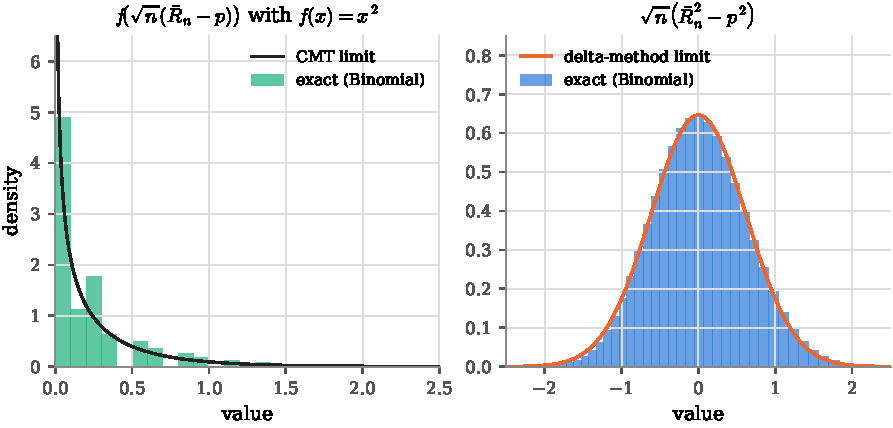
\includegraphics[width=\textwidth]{fig_cmt_pitfall}
\caption{Two different random variables for $f(x) = x^2$ in the kiss model, $p = 0.645$, $n = 124$. Left: $(\sqrt{n}(\bar{R}_n - p))^2$ with its CMT limit (black curve). Right: $\sqrt{n}(\bar{R}_n^2 - p^2)$ with its delta-method limit (orange curve). The bars are the exact Binomial distribution of $n\bar{R}_n$, binned.}
\label{fig:cmtpitfall}
\end{figure}

\section{The delta method}
\label{sec:delta-method}

The delta method is what you need when you're taking the limit of something like $\sqrt{n} \left( g(\bar{X}_n) - g(\mu) \right)$: you know the CLT for $\bar{X}_n$, and you want the CLT for a function of it.

\begin{theorem}[Delta method]
\label{thm:delta}
Let $(Z_n)_{n \geq 1}$ be a sequence of r.v.s such that:
\[
\sqrt{n} (Z_n - \theta) \convd \Gauss(0, \sigma^2),
\]
for some $\theta \in \real$ and $\sigma^2 > 0$.
A sequence like $(Z_n)_{n \geq 1}$ that satisfies this condition is said to be \textit{asymptotically normal around} $\theta$, and $\sigma^2$ is its asymptotic variance.
Let $g: \real \to \real$ be continuously differentiable at the point $\theta$.
Then:
\begin{enumerate}[nosep]
\item $g(Z_n) \convp g(\theta)$;
\item $(g(Z_n))_{n \geq 1}$ is also asymptotically normal, around $g(\theta)$;
\item more precisely,
\[
\sqrt{n} \left( g(Z_n) - g(\theta) \right) \convd \Gauss \left( 0, \, g'(\theta)^2 \sigma^2 \right).
\]
\end{enumerate}
\end{theorem}

\begin{intuition}[a differentiable function is locally linear]
\Cref{fig:delta} is the whole idea.
It is drawn for $g(x) = 1/x$ with the numbers of the subway example below, $\theta = 6.23$ and $\sigma/\sqrt{n} = 0.78$; the dotted lines map $\theta \pm 2\sigma/\sqrt{n}$ across.
For large $n$, $Z_n$ sits in a narrow Gaussian blob of width $\sigma/\sqrt{n}$ around $\theta$.
On a blob that narrow, the curve $g$ is indistinguishable from its tangent line at $\theta$, which has slope $g'(\theta)$.
A linear function maps a Gaussian to a Gaussian, shifting the center to $g(\theta)$ and multiplying the width by the slope.
So $g(Z_n)$ sits in a Gaussian blob of width $\abs{g'(\theta)} \, \sigma / \sqrt{n}$ around $g(\theta)$, which is statement (3).
Where $g$ is steep, errors in $Z_n$ are amplified; where it's flat, they're damped.
\end{intuition}

\begin{figure}[htbp]
\centering
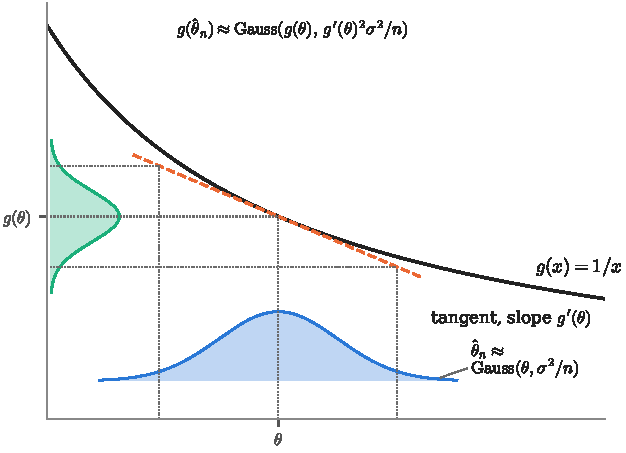
\includegraphics[width=0.78\textwidth]{fig_delta_method}
\caption{The delta method for $g(x) = 1/x$, $\theta = 6.23$, $\sigma/\sqrt{n} = 0.78$: the input Gaussian in blue on the horizontal axis, its image in green on the vertical axis, the tangent at $\theta$ dashed in orange, and dotted guides at $\theta \pm 2\sigma/\sqrt{n}$.}
\label{fig:delta}
\end{figure}

\coreproof{The mean value theorem \toolkit{sec:math-mvt} writes $g(Z_n) - g(\theta)$ as a slope times $Z_n - \theta$. The slope converges in probability to $g'(\theta)$ (CMT), and $\sqrt{n}(Z_n - \theta)$ converges in distribution (the assumption); Slutsky multiplies the two.}
\begin{proof}
By the mean value theorem there's a point $\tilde{\theta}_n$ between $Z_n$ and $\theta$ such that
\[
g(Z_n) - g(\theta) = g'(\tilde{\theta}_n)(Z_n - \theta).
\]
Multiply through by $\sqrt{n}$:
\[
\sqrt{n} \left( g(Z_n) - g(\theta) \right) = g'(\tilde{\theta}_n) \cdot \sqrt{n}(Z_n - \theta).
\]
Now take the two factors in turn.
First, $Z_n \convp \theta$: by Slutsky, $Z_n - \theta = \frac{1}{\sqrt{n}} \cdot \sqrt{n}(Z_n - \theta) \convd 0 \cdot \Gauss(0, \sigma^2) = 0$, and convergence in distribution to a constant is convergence in probability (\cref{prop:convd-constant}).
This proves (1) via the CMT, and since $\tilde{\theta}_n$ is squeezed between $Z_n$ and $\theta$, also $\tilde{\theta}_n \convp \theta$, hence $g'(\tilde{\theta}_n) \convp g'(\theta)$ by the CMT and the continuity of $g'$ at $\theta$.
Second, $\sqrt{n}(Z_n - \theta) \convd \Gauss(0, \sigma^2)$ by assumption.
Slutsky's multiplicative property with $y = g'(\theta)$ gives
\[
g'(\tilde{\theta}_n) \cdot \sqrt{n}(Z_n - \theta) \convd g'(\theta) \cdot \Gauss(0, \sigma^2) = \Gauss(0, g'(\theta)^2 \sigma^2),
\]
which is (3), and (2) is (3) read as a sentence.
\end{proof}

The proof is three lines because Slutsky and the CMT did the work in advance.
Note that nothing requires $g$ to be invertible or monotone; $g(x) = \sqrt{2} \sin x$ is a perfectly good choice.
Note also that the asymptotic variance $g'(\theta)^2 \sigma^2$ generally depends on the unknown $\theta$, even when $\sigma^2$ doesn't; the plug-in trick of the previous section handles that.

\begin{worked}[inter-arrival times of the T]
You observe the times between arrivals of the subway at Kendall, $T_1, \ldots, T_n$, and model them as i.i.d.\ $\Expo(\lambda)$, so $\E[T_1] = 1/\lambda$ and $\var(T_1) = 1/\lambda^2$.
The natural estimator of $\lambda$ is $\hat{\lambda} = 1/\bar{T}_n$.
\begin{itemize}[nosep]
\item \textit{Consistency.} $\bar{T}_n \convp 1/\lambda$ by the Law of Large Numbers, so $\hat{\lambda} = 1/\bar{T}_n \convp \lambda$ by the CMT ($f(x) = 1/x$ is continuous at $1/\lambda > 0$).
\item \textit{The CLT for $\bar{T}_n$.} $\sqrt{n} \left( \bar{T}_n - \frac{1}{\lambda} \right) \convd \Gauss(0, \lambda^{-2})$.
\item \textit{The delta method for $\hat{\lambda}$.} Take $g(x) = 1/x$, so $g'(x) = -1/x^2$ and $g'(1/\lambda)^2 = \lambda^4$. Then
\[
\sqrt{n} \left( \hat{\lambda} - \lambda \right) \convd \Gauss \left( 0, \, \lambda^4 \cdot \lambda^{-2} \right) = \Gauss(0, \lambda^2).
\]
\end{itemize}
With $n = 64$ and $\bar{T}_n = 6.23$ minutes: $\hat{\lambda} = 0.1605$ per minute, and the standard error of $\hat{\lambda}$ (the standard deviation $\lambda/\sqrt{n}$ of its approximating Gaussian, with $\hat{\lambda}$ plugged in for $\lambda$) is about $0.020$.
So $\lambda$ is pinned down to roughly $0.16 \pm 0.04$, which becomes the plug-in confidence interval $[0.12, 0.20]$ of \cref{ch:confidence-intervals}.
\end{worked}

\begin{worked}[odds in the kiss experiment]
The odds of turning right are $\omega = p/(1-p)$, estimated by $\hat{\omega} = \bar{R}_n/(1 - \bar{R}_n)$.
With $g(p) = p/(1-p)$ you get $g'(p) = 1/(1-p)^2$, and the CLT gives asymptotic variance $p(1-p)$ for $\bar{R}_n$, so
\[
\sqrt{n} \left( \hat{\omega} - \omega \right) \convd \Gauss \left( 0, \, \frac{p(1-p)}{(1-p)^4} \right) = \Gauss \left( 0, \, \frac{p}{(1-p)^3} \right).
\]
At $p = 0.645$ and $n = 124$: $\hat{\omega} = 1.82$ and the standard error is $\sqrt{0.645/0.355^3/124} \approx 0.34$.
The derivative $1/(1-p)^2 \approx 7.9$ is large, so the odds are estimated far less precisely, in absolute terms, than the proportion they're computed from: a steep $g$ amplifies the error.
\Cref{fig:steepflat} puts this next to a flat $g$, where the same input error nearly disappears.
The input on both sides is $\bar{R}_n \approx \Gauss(p, p(1-p)/n)$ with standard deviation $0.043$.
On the left, the odds have slope $7.9$ at $p = 0.645$, and the output standard deviation is $7.9 \times 0.043 = 0.34$.
On the right, the variance $g(p) = p(1-p)$ has slope $-0.29$ there, and the output standard deviation is $0.29 \times 0.043 = 0.012$.
Same data and the same precision in $p$; the delta method's $\abs{g'(\theta)}$ is the whole difference in the precision of $g(p)$.
\end{worked}

\begin{figure}[htbp]
\centering
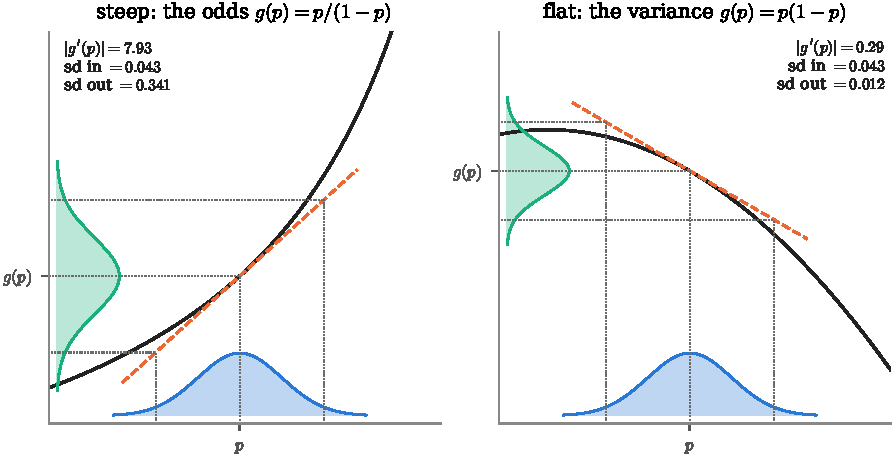
\includegraphics[width=\textwidth]{fig_delta_steep_flat}
\caption{The input $\bar{R}_n \approx \Gauss(p, p(1-p)/n)$, in blue on the horizontal axis, pushed through two functions, with the output in green on the vertical axis and the tangent at $p$ dashed in orange. Left: the odds $g(p) = p/(1-p)$. Right: the variance $g(p) = p(1-p)$.}
\label{fig:steepflat}
\end{figure}

\begin{bridge}[propagation of error]
If you took a laboratory course you met the rule `if $y = g(x)$ and $x$ has uncertainty $\delta x$, then $y$ has uncertainty $\delta y \approx \abs{g'(x)} \, \delta x$'.
The delta method is that rule for standard errors, with a theorem attached:
\[
\se \left( g(\ethn) \right) \approx \abs{g'(\theta)} \, \se(\ethn), \qquad \se(\ethn) = \frac{\sigma}{\sqrt{n}}.
\]
It also says what the lab rule leaves out: the transformed estimate isn't just `uncertain by $\delta y$', it's approximately Gaussian, so you can attach a probability to the error bar.
\end{bridge}

\begin{remark}
When $g'(\theta) = 0$ the theorem still holds but says only that $\sqrt{n}(g(Z_n) - g(\theta)) \convd 0$, that is, the error of $g(Z_n)$ is of smaller order than $1/\sqrt{n}$.
To see the actual limit you magnify by $n$ instead of $\sqrt{n}$ and get a second-order expansion: $n(g(Z_n) - g(\theta)) \convd \frac{\sigma^2 g''(\theta)}{2} \chi^2_1$.
No result later in this book needs this case.
\end{remark}

\begin{remark}[Vector versions]
Everything in this chapter has a version for vectors, with a covariance matrix in place of $\sigma^2$ and a matrix of partial derivatives in place of $g'(\theta)$.
If $\sqrt{n}(Z_n - \theta) \convd \Gauss_d(0, \Sigma)$ and $g: \real^d \to \real^k$ is continuously differentiable at $\theta$, with $\nabla g(\theta)$ the $d \times k$ matrix of partial derivatives, then
\[
\sqrt{n} \left( g(Z_n) - g(\theta) \right) \convd \Gauss_k \left( 0, \, \nabla g(\theta)^\top \Sigma \, \nabla g(\theta) \right),
\]
and the multivariate CLT says that the vector of sample means of i.i.d.\ vectors with covariance $\Sigma$ satisfies the hypothesis with $\Sigma$ itself.
The proofs are the ones above with matrices in place of numbers.
The method of moments (\cref{ch:mom-mestimation}) and the chi-squared goodness-of-fit test (\cref{ch:gof}) use these, and the book states them again there in the form each needs.
\end{remark}

\begin{bridge}[the confidence interval for an odds ratio]
Courses in biostatistics and epidemiology teach a confidence interval for an odds ratio: the log of the estimated odds ratio plus or minus $1.96\sqrt{1/a + 1/b + 1/c + 1/d}$, with $a, b, c, d$ the four counts of the two-by-two table, exponentiated at both ends.
The square root is the delta method.
For one group with $S$ successes in $n$ trials, the log odds $g(p) = \log\big(p/(1-p)\big)$ has $g'(p) = 1/\big(p(1-p)\big)$, so \cref{thm:delta} gives it approximate variance $g'(p)^2 \, p(1-p)/n = \big(1/p + 1/(1-p)\big)/n$, which with $\hat{p} = S/n$ plugged in is $1/S + 1/(n - S)$.
For the kiss data the log odds of turning right is $\log(80/44) = 0.598$ with standard error $\sqrt{1/80 + 1/44} = 0.188$, and exponentiating the ends of $0.598 \pm 1.96 \times 0.188$, which keeps the level (\cref{sec:ci-subway}), gives $[1.26, 2.63]$ for the odds.
An odds ratio compares two independent groups, so its log is the difference of two independent log odds, and the variance of that difference adds all four reciprocals.
\end{bridge}

\section{Where the limit theorems are used in the rest of the book}
\label{sec:conv-where-used}

Every asymptotic statement in the later chapters is one of the facts of \cref{ch:lln,ch:clt} or this chapter in disguise, with two exceptions the table names, both stated without proof (Donsker's theorem about the whole empirical CDF, behind the Kolmogorov--Smirnov test, and the Bernstein--von Mises theorem of \cref{ch:bayes-intro}).
The table says which.
`LLN' means the Law of Large Numbers (\cref{thm:wlln}), `CLT' the Central Limit Theorem (\cref{thm:clt}), `CMT' the continuous mapping theorem (\cref{thm:cmt}), `Slutsky' \cref{thm:slutsky}, and `delta' the delta method (\cref{thm:delta}).

\begin{center}
\small
\begin{tabular}{@{}>{\raggedright\arraybackslash}p{2.55in}>{\raggedright\arraybackslash}p{0.9in}>{\raggedright\arraybackslash}p{2.45in}@{}}
\toprule
Result & Chapter & Rests on \\
\midrule
Consistency of $\bar{X}_n$, $\hat{p}$, and any estimator built from an average & \cref{ch:estimators} & LLN, then CMT for functions of averages \\[3pt]
Asymptotic confidence intervals; the plug-in interval & \cref{ch:confidence-intervals} & CLT; Slutsky for replacing $p$ by $\hat{p}$ in the standard error \\[3pt]
Confidence interval for $1/\bar{T}_n$ and other transformed estimators & \cref{ch:confidence-intervals} & delta \\[3pt]
Level and $p$-value of a test built on a standardized average & \cref{ch:tests-foundations} & CLT, Slutsky \\[3pt]
Consistency of the maximum likelihood estimator & \cref{ch:mle-properties} & LLN applied to the average log-likelihood, plus the KL divergence argument \\[3pt]
Asymptotic normality of the MLE, with variance $1/I(\theta)$ & \cref{ch:mle-properties} & CLT applied to the average score, then a Taylor expansion exactly as in the delta method proof, with Fisher information as the slope \\[3pt]
Method of moments: consistency and asymptotic variance & \cref{ch:mom-mestimation} & LLN, then the (multivariate) delta method \\[3pt]
Wald test & \cref{ch:wald-lrt} & asymptotic normality of the MLE, Slutsky for the estimated information, CMT (squaring gives a $\chi^2$) \\[3pt]
Likelihood ratio test (Wilks' theorem) & \cref{ch:wald-lrt} & a second-order Taylor expansion, the same device as the delta method, plus Slutsky \\[3pt]
Score test & \cref{ch:wald-lrt} & multivariate CLT applied to the score, then CMT \\[3pt]
$t$-test & \cref{ch:t-test} & nothing here: exact for Gaussian data (Cochran's theorem) \\[3pt]
Chi-squared goodness-of-fit test & \cref{ch:gof} & multivariate CLT for the rotated standardized deviations of the counts, then CMT; with estimated parameters, the nuisance-parameter theorem of \cref{ch:wald-lrt} \\[3pt]
Kolmogorov--Smirnov and Lilliefors tests & \cref{ch:ks} & Glivenko--Cantelli (a uniform LLN), proved there from the LLN at finitely many points; Donsker's theorem (a CLT for the whole empirical CDF), stated without proof \\[3pt]
Bayesian posteriors concentrate on the truth (proved for Beta priors); Bernstein--von Mises & \cref{ch:bayes-intro} & LLN and Chebyshev for the concentration; Bernstein--von Mises stated, not proved \\[3pt]
Inference for least squares with non-Gaussian errors & \cref{ch:regression-multi} & CLT (exact $t$ and $F$ when errors are Gaussian) \\[3pt]
Asymptotic normality of GLM estimates & \cref{ch:glm-links} & the MLE result again \\[3pt]
Sample covariance converges to the true covariance & \cref{ch:pca} & LLN entrywise, then CMT for the eigenvectors \\
\bottomrule
\end{tabular}
\end{center}

\section{What comes next}
\label{sec:tools-next}

Every limit in these three chapters landed on the same distribution.
\Cref{ch:gaussian} collects what the rest of the book needs about it: the density, the three properties that let you standardize anything Gaussian, how to turn a Gaussian probability into a table lookup, and this book's convention for quantiles, which is the notation every confidence interval and test from \cref{ch:confidence-intervals} on is written in.
If you know the Gaussian well, the quantile section is the one part not to skip.

\section{Summary}
\label{sec:tools-summary}

\begin{itemize}[nosep]
\item For convergence in probability (and almost surely), limits add, multiply and divide like limits of numbers. For convergence in distribution they do not: the marginal limits of $X_n$ and $Y_n$ don't determine the limit of $X_n + Y_n$.
\item \textbf{Slutsky's theorem:} if $X_n \convd X$ and $Y_n \convp y$ with $y$ a constant, then $X_n + Y_n \convd X + y$, $X_n Y_n \convd yX$ and $X_n / Y_n \convd X/y$. This justifies every plug-in: replacing $\sigma$ by $s$, or $p$ by $\hat{p}$, in a standard error.
\item \textbf{Continuous mapping theorem:} $X_n \to X$ in any of the three modes implies $f(X_n) \to f(X)$ in the same mode, for $f$ continuous at the limit. Consistency survives transformations. What it does not give you is the limit of $\sqrt{n}(f(\bar{X}_n) - f(\mu))$; that is the delta method's job.
\item \textbf{Delta method:} if $\sqrt{n}(Z_n - \theta) \convd \Gauss(0, \sigma^2)$ and $g$ is continuously differentiable at $\theta$, then $\sqrt{n}(g(Z_n) - g(\theta)) \convd \Gauss(0, g'(\theta)^2 \sigma^2)$. A narrow Gaussian blob pushed through a smooth curve comes out Gaussian, with its width multiplied by the slope. This is propagation of error with a theorem attached.
\end{itemize}

\section{Exercises}
\label{sec:tools-exercises}

\begin{exercise}
Let $\Xton \iid \Bern(p)$. Use the delta method to find the asymptotic distribution of $\sqrt{n} \left( \bar{X}_n(1 - \bar{X}_n) - p(1-p) \right)$. For which $p$ does the delta method fail to give a Gaussian limit, and why?
\end{exercise}
\begin{solution}
With $g(p) = p(1-p)$, $g'(p) = 1 - 2p$, and the CLT gives asymptotic variance $p(1-p)$ for $\bar{X}_n$, so the limit is $\Gauss(0, (1-2p)^2 p(1-p))$. At $p = \frac12$ the derivative is $0$ and the limit is degenerate: the sample variance of a fair coin is estimated with error of order $1/n$ rather than $1/\sqrt{n}$, and the second-order remark of \cref{sec:delta-method} applies.
\end{solution}

\begin{exercise}
Let $\Xton \iid \Expo(\lambda)$. Show that $\sqrt{n}(\log \bar{X}_n + \log \lambda) \convd \Gauss(0, 1)$, whatever $\lambda$ is. Why might a statistician prefer to build a confidence interval for $\log(1/\lambda)$ rather than for $1/\lambda$?
\end{exercise}
\begin{solution}
The CLT gives $\sqrt{n}(\bar{X}_n - 1/\lambda) \convd \Gauss(0, 1/\lambda^2)$. With $g(x) = \log x$, $g'(1/\lambda) = \lambda$, so the asymptotic variance of $\log \bar{X}_n$ is $\lambda^2 \cdot \lambda^{-2} = 1$, free of $\lambda$. A limit whose variance doesn't depend on the unknown parameter needs no plug-in: the interval $\log \bar{X}_n \pm 1.96/\sqrt{n}$ for $\log(1/\lambda)$ has asymptotic level $95\%$ with no further work, and can be exponentiated afterwards. This is called a variance-stabilizing transformation.
\end{solution}

\begin{exercise}
Let $\Xton \iid \Bern(p)$ with $0 < p < 1$. Show that
\[
\sqrt{n}\,\frac{\bar{X}_n - p}{\sqrt{\bar{X}_n(1 - \bar{X}_n)}} \convd \Gauss(0,1),
\]
naming the theorem used at each step.
\end{exercise}
\begin{solution}
By the CLT, $\sqrt{n}(\bar{X}_n - p)/\sqrt{p(1-p)} \convd \Gauss(0,1)$. By the LLN, $\bar{X}_n \convp p$, and $x \mapsto \sqrt{p(1-p)/(x(1-x))}$ is continuous at $p$, so by the continuous mapping theorem $\sqrt{p(1-p)/(\bar{X}_n(1-\bar{X}_n))} \convp 1$. Slutsky's multiplicative property with $y = 1$ gives the product's limit, $1 \cdot \Gauss(0,1)$.
\end{solution}
